%============================================================================
% tento soubor pouzijte jako zaklad
% (c) 2008 Michal Bidlo
% E-mail: bidlom AT fit vutbr cz
%============================================================================
% kodovaní: utf8 (zmena prikazem iconv, recode nebo cstocs)
%----------------------------------------------------------------------------
% zpracování: make, make pdf, make desky, make clean
% připomínky posílejte na e-mail: bidlom AT fit.vutbr.cz
% vim: set syntax=tex
%============================================================================
\documentclass[english]{jtulak} % odevzdani do wisu - odkazy, na ktere se da klikat
%\documentclass[cover,print]{fitthesis} % pro tisk - na odkazy se neda klikat
%\documentclass[english,print]{fitthesis} % pro tisk - na odkazy se neda klikat
%      \documentclass[english]{fitthesis}
% * Je-li prace psana v anglickem jazyce, je zapotrebi u tridy pouzit 
%   parametr english nasledovne:
%      \documentclass[english]{fitthesis}
% * Neprejete-li si vysazet na prvni strane dokumentu desky, zruste 
%   parametr cover

% zde zvolime kodovani, ve kterem je napsan text prace
% "latin2" pro iso8859-2 nebo "cp1250" pro windows-1250, "utf8" pro "utf-8"
%\usepackage{ucs}
\usepackage[utf8]{inputenc}
%\usepackage[T1, IL2]{fontenc}
\usepackage{url}
\DeclareUrlCommand\url{\def\UrlLeft{<}\def\UrlRight{>} \urlstyle{tt}}

%zde muzeme vlozit vlastni balicky

\usepackage{sidecap}
\usepackage{listings}
\usepackage{syntonly}
\usepackage{wrapfig}
\usepackage{csquotes}
%\syntaxonly

% =======================================================================
% balíček "hyperref" vytváří klikací odkazy v pdf, pokud tedy použijeme pdflatex
% problém je, že balíček hyperref musí být uveden jako poslední, takže nemůže
% být v šabloně

\ifx\pdfoutput\undefined % nejedeme pod pdflatexem
	\usepackage[dvips]{color, graphicx}
	\usepackage[tex4ht]{hyperref}
\else
  \ifNotPrint
    \usepackage{color}
    \usepackage[unicode,colorlinks,hyperindex,plainpages=false,pdftex]{hyperref}
    \definecolor{links}{rgb}{0.4,0.5,0}
    \definecolor{anchors}{rgb}{1,0,0}
    \hypersetup{
      colorlinks,
      citecolor=Green,
      %linkcolor=links,
      %urlcolor=links
      }
    \def\AnchorColor{anchors}
    \def\LinkColor{links}
    \def\pdfBorderAttrs{/Border [0 0 0] }  % bez okrajů kolem odkazů
    \pdfcompresslevel=9
  \fi
\fi

%Informace o praci/projektu
%---------------------------------------------------------------------------
\projectinfo{
  %Prace
  project=DP,            %typ prace BP/SP/DP/DR
  year=2017,             %rok
  date=\today,           %datum odevzdani
  %Nazev prace
  title.cs={Refaktoring a verifikace kódu mkfs xfs},  %nazev prace v cestine
  title.en={Refactoring and Verification of the Code of mkfs xfs}, %nazev prace v anglictine
  %Autor
  author={Jan Ťulák},   %jmeno prijmeni autora
  author.title.p=Bc., %titul pred jmenem (nepovinne)
  %author.title.a=PhD, %titul za jmenem (nepovinne)
  %Ustav
  department=UITS, % doplnte prislusnou zkratku: UPSY/UIFS/UITS/UPGM
  %Skolitel
  supervisor= Tomáš Vojnar, %jmeno prijmeni skolitele
  supervisor.title.p=prof. Ing.,   %titul pred jmenem (nepovinne)
  supervisor.title.a={Ph.D.},    %titul za jmenem (nepovinne)
  %Klicova slova, abstrakty, prohlaseni a podekovani je mozne definovat 
  %bud pomoci nasledujicich parametru nebo pomoci vyhrazenych maker (viz dale)
  %===========================================================================
  %Klicova slova
  keywords.cs={klicova slova}, %klicova slova v ceskem jazyce
  keywords.en={keywords}, %klicova slova v anglickem jazyce
  %Abstract
  % abstrakt v ceskem jazyce
  abstract.cs={
	  Tato práce popisuje průběh a smysl refaktoringu mkfs.xfs programu
	  a následně srovnává řadu nástrojů pro statickou analýzu a
	  verifikaci na refaktorovaném kódu.},
  % abstrakt v anglickem jazyce
  abstract.en={
	  This work describes the progress and the reason of a mkfs.xfs
	  refactoring. Then it compares multiple tools for static analysis
	  and verification of the refactored code.
  }, 
  %Prohlaseni
  declaration={
	Hereby I declare that I wrote this work on my own and all
	used sources are stated and correctly noted as citations.
  },
  %Podekovani (nepovinne)
  acknowledgment={I want to thanks to my manager Steven Whitehouse, my
  colleagues at Red Hat, to David Chinner, maintainer of XFS, and to
  everyone in XFS community.}, % nepovinne
  % Rozsireny abstrakt v ceskem jazyce
  abstractext.cs={
	Rozšířený abstrakt v češtině, protože to prý práce v AJ
	musí mít.
  },
}

%Abstrakt (cesky, anglicky)
%\abstract[cs]{Do tohoto odstavce bude zapsán výtah (abstrakt) práce v českém jazyce.}
%\abstract[en]{Do tohoto odstavce bude zapsán výtah (abstrakt) práce v anglickém jazyce.}

%Klicova slova (cesky, anglicky)
\keywords[cs]{XFS, refaktoring, formální analýza, formální verifikace,
Coverity, CPAChecker.}
\keywords[en]{XFS, refactoring, formal analysis, formal verification,
Coverity, CPAChecker.}

%Prohlaseni
%\declaration{Prohlašuji, že jsem tuto bakalářskou práci vypracoval samostatně pod vedením pana X...
%Další informace mi poskytli...
%Uvedl jsem všechny literární prameny a publikace, ze kterých jsem čerpal.}

%Podekovani (nepovinne)
%\acknowledgment{V této sekci je možno uvést poděkování vedoucímu práce a těm, kteří poskytli odbornou pomoc
%(externí zadavatel, konzultant, apod.).}

%%%%%%%%%%%%%%%%%%%%%%%%%

% my macro for function declaration
\newcommand{\FunctionDeclareNE}[4]{%
  \noindent
  \ifdefined\hyperref
    \phantomsection
  \fi
  \label{fnt:#2}
  \textbf{{\em #1} {\tt #2} ( {\em #3} ) }-- {#4}
  \endgroup}
% because underscore is a special character and has to be escaped
% but escaped sequences must not be in \label
\def\FunctionDeclare{\begingroup 
\catcode`\_=12
\FunctionDeclareNE}

% my macro for linking to a function declaration
\newcommand{\functionNE}[1]{%
  \ifdefined\hyperref
    \hyperref[fnt:#1]{\tt #1}%
  \else
    {\tt #1}%
  \fi
\endgroup}
% because underscore is a special character and has to be escaped
% but escaped sequences must not be in \label
\def\function{\begingroup 
\catcode`\_=12
\functionNE}

%%%%%%%%%%%%%%%%%%%%%
% my macro for function declaration
\newcommand{\MachineDeclareNE}[4]{%
  \noindent
  \ifdefined\hyperref
    \phantomsection
  \fi
  \label{machines:#1}
  \textbf{#1}\\
    CPU: {\it #2}\\
    RAM: {\it #3}\\
    Notes: {\it #4}\\
  \endgroup}
% because underscore is a special character and has to be escaped
% but escaped sequences must not be in \label
\def\machineDeclare{\begingroup 
\catcode`\_=12
\MachineDeclareNE}

\newcommand{\machineNE}[1]{%
  \ifdefined\hyperref
    \hyperref[machines:#1]{\it #1}%
  \else
    {\it #1}%
  \fi
\endgroup}
% because underscore is a special character and has to be escaped
% but escaped sequences must not be in \label
\def\machine{\begingroup 
\catcode`\_=12
\machineNE}


%%%%%%%%%%%%%%%%%%%%%

\begin{document}

\pagenumbering{Alph}
  % Vysazeni titulnich stran
  % ----------------------------------------------
  \maketitle
  
  % Obsah
  % ----------------------------------------------
\pagenumbering{arabic}
  \tableofcontents
  
  % Seznam obrazku a tabulek (pokud prace obsahuje velke mnozstvi obrazku, tak se to hodi)
  % \listoffigures
  % \listoftables 

  % Text prace
  % ----------------------------------------------
  %
%==================================
% (c) Jan Tulak, 2017

\chapter{Introduction}\label{chap:introduction}


In projects with long life, even an initially clean code can become messy and complicated. Moreover when we speak about open-source projects where the original creators left yers ago and new people of various capabilities and knowledge continue the development.

In such a projects, new functionality is added to the existing code with minimal changes of the rest of the project. This may simplify the merging of these changes, as any responsible person can easily understand what the change does. But on the other side, in long term, it turns the code into so-called spaghetti.

The result is increasingly more difficult to maintain and test, and as a single functionality can be spread over many portions of the project, any change requires more and more attention and time.

XFSprogs, a package of tools for XFS filesystem, is such a project. While the filesystem itself is getting some strict eye from the Linux kernel community nowdays, the tools like {\tt mkfs.xfs}\footnote{Formats a partition as XFS.}, {\tt fsck.xfs}\footnote{Checks and repairs errors in an existing XFS filesystem.} and others are not so publicly exposed and gets a lot less attention. From my experience with working on this project, it happens that only one or two persons other than the author of a patch read it, and miss some subtle side effect the change has. Sometimes, the large set of tests XFS maintains captures this bug, sometimes it doesn't and it is noticed much later.

On this point, it is important to highlight that despite the naming
convention, each {\tt mkfs} tool is completely independent project and, for
example, {\tt mkfs.xfs} and {\tt mkfs.ext4} don't share any code except
system libraries.

Some parts of this code are more than 20 years old (see chapter 1 for more detailed history of XFS) and in the need of intensive cleaning. The tests suite (project xfstests) maintains hundreds of more or less complex tests, but these are limited in what they can detect as they usually work in this way: make a filesystem, then test that, so many errors in {\tt mkfs.xfs} are difficult to capture or notice. XFS also uses an automatic static analysis from Coverity, which is useful, but the project has no good data on the reliability of this analysis.

With the approval of David Chinner, the maintainer of XFS, I began the
refactoring of mkfs.xfs, which was most in due. The goal of this work is to repay the technical debt accumulated over the years and then verify how effective the currently used tests and analysis are on at least a part of the code. At the same time, this work can be also seen as a review of how well can various analysis and verification methods do on a real, in production used code.

The refactoring was done in two parts. One set of changes was merged into upstream in June 2016 (xfsprogs 4.7), the other set is, at the time of writing, still waiting for a review:
\begin{itemize}
\item Before the beginning of refactoring -- xfsprogs 4.6.
\item After merging the first part -- xfsprogs 4.7.
\item Before merging the second part -- xfsprogs 4.9 at the time of writing.
\item After applying the second part -- not yet merged, changes only in a local repository.
\end{itemize}

This work is structured as follows: First, information about XFS and
mkfs.xfs are provided in the first chapter. In the following, third chapter, we look
at the refactoring done and discuss the changes. After that, another
chapter is dedicated to explaining formal analysis and verification,
describing common techniques, and we points out notable tools. And finally
in the fifth chapter, we discuss possible approaches for the analysis and
verification specifically of mkfs.xfs.


%==================================
% (c) Jan Tulak, 2017
%%%%%%%%%%%%%%%%%%%%%%%%%%%%%%%%%%%%%%%%%%%%%%%%%%%%%%%%%%%%%%%%%%%%%%%%%%%%%

\chapter{XFS filesystem} \label{chap:xfs}
%----------------------------------------------------------------------

XFS is a journaling filesystem created by SGI in 1993. The new filesystem, intended as a powerful replacement of EFS with the expectation of growing amount of data in the future was first released in IRIX 5.3. Linux port began in 1999 and since 2002 is XFS accessible in the mainline Linux Kernel~\cite[Chap. 1.2, 1.3]{xfsHistory}.

\begin{table}[h]
\begin{tabular}{|l||r|r|r|r|}
\hline
& ext3 & ext4 & XFS & NTFS \\

\hline
\hline
max fs size & $16$ TiB & $16$ TiB & $16$ EiB& $256$ TiB\\
\hline
max file size & $8$ TiB & $16$ TiB & $8$ EiB & $256$ TiB\\
\hline
max files & $2^{32}$ & $2^{32}$& $2^{64}$ & $2^{32}$\\
\hline
date resolution & $1$ s & $1$ ns & $1$ ns & $100$ ns\\
\hline
\end{tabular}
\caption{Comparison of various filesystems and their limits. Sources:~\cite{inodesInLinux,NTFS1,NTFS2,NTFSfiletime,XFSforLinux}.}
\label{tab:xfs:comparison}
\end{table}



Because of its capabilities, XFS used also by well known institutions like CERN or Fermilab~\cite{XFSforLinux} for storing large amounts of data. Unlike most of other Linux filesystems, XFS is a 64bit fs, meaning it provides far greater limits for storage and file size\footnote{At least matured ones. Newer filesystems, like Btrfs, are also 64bit, but have not yet reached stability required in business sector.}, but its architecture also offer great scalability in terms of parallel I/O.

XFS as a whole is separated into three main projects: First, there is the XFS filesystem itself, in the form of a kernel module. Then a set of tools in a package called xfsprogs is tightly connected with XFS filesystem and contains programs useful or necessary for creation and manipulation of the filesystem. Among the tools included are {\tt mkfs.xfs}, on which this thesis is focused, but also other tools: {\tt fsck.xfs}, {\tt xfs\_io}, {\tt xfs\_growfs}, et cetera. And finally, there are xfstests, which is a test suite containing hundreds of shell scripts that verifying the behaviour of entire XFS chain (from mkfs to the kernel code). This project is also partially used by other filesystems. There are among others tests for ext4, overlay fs and btrfs.

Except for the xfstests test suite, xfsprogs also uses an automatical static analysis from Coverity~\cite{CoverityXfsprogs}. However, to see detailed information and defects there, one must be approved by existing members of the project.


%======================================================================
\section{XFS Architecture overview}\label{chap:xfs:overview}
%----------------------------------------------------------------------

When a XFS partition is formated, up to three areas are created on the disk: Data section is always present. An optional real-time section is omitted by default. Log section has to exist always but can be placed on a different device. The data part is then in fact split into multiple de facto independent filesystems called Allocation Groups, that handle space allocation and allows for higher parallelism, as most operations can be done on each Allocation Group independently on the others. The log section can be also internal to each of the Allocation Groups.

As each Allocation Group is a de facto standalone filesystem, each contains
the superblock and block and inode allocations and the only global
information, maintained by the first (primary) AG is free space and total
inode counts across the whole filesystem as can be seen
on figure~\ref{fig:xfs:primaryAG}.

\begin{figure}
  \centering
 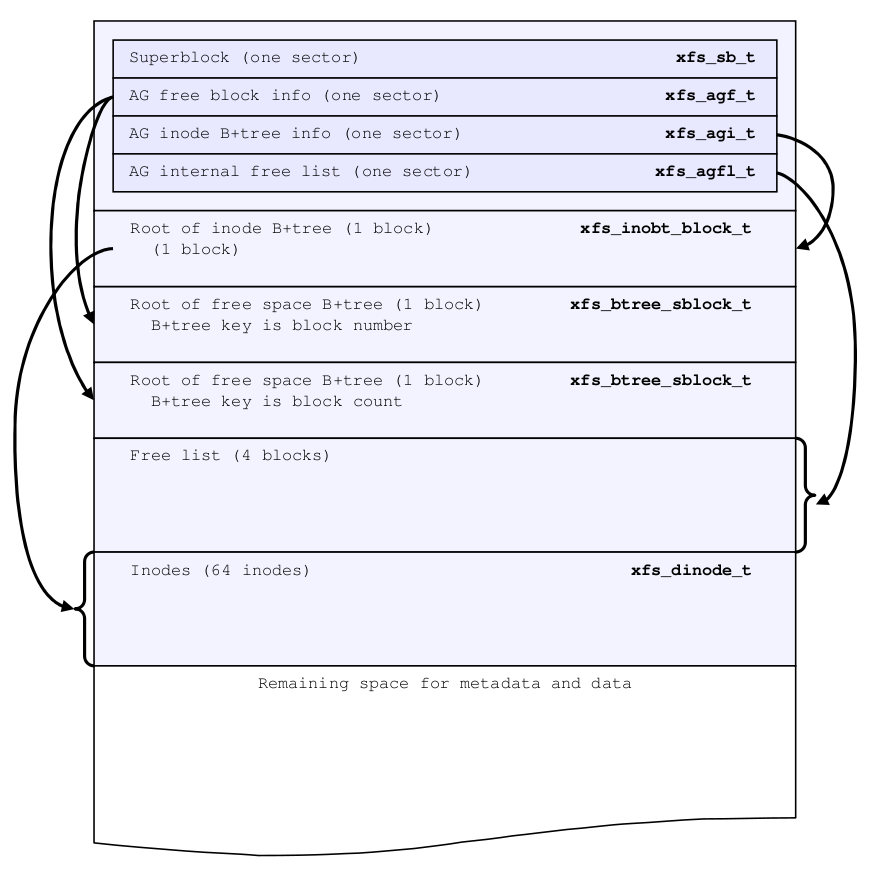
\includegraphics[width=13cm,keepaspectratio]{fig/primary-ag} % Or .pdf
 \caption{Primary AG right after mkfs~\cite[Ch. 3]{xfsStructure}.}
\label{fig:xfs:primaryAG}
\end{figure}
	
Real-time section is dedicated for files with a real-time attribute bit set, and operations with these files should have predictable latencies~\cite{xfsRealtime}. Log section is used to recover from situations like power failure on the next mount~\cite{xfsStructure,xfsman}.

When created on striped RAID\footnote{Striped RAID is e.g. RAID 0, where logically sequential data are split into a number of physical blocks and written on multiple disks interleaved. For a RAID 0 on two drives it means that odd blocks are located on one drive and even blocks on the other.}, XFS can be informed about it and align all allocations and size to the stripe unit to maximize speed.


%======================================================================
\section{mkfs.xfs}\label{chap:xfs:mkfs}
%----------------------------------------------------------------------

This chapter describes in a greater detail the mkfs.xfs program itself, located
in file {\tt mkfs/mkfs\_xfs.c}, from user point of view. For information about
its implementation, see chapter~\ref{chap:refactoring:initialcodebase}. This
tool creates a new XFS filesystem with given properties. It is, as is usual for
core Unix utilities, a non-interactive program which accepts multiple arguments
when called and prints out the properties of the newly created filesystem if
successful, or prints an error and usage help when an error occurs.

\begin{lstlisting}[frame=none, basicstyle=\footnotesize\ttfamily, language=Bash, numbers=none, numberstyle=\tiny\color{black},caption= {Synopsis of mkfs.xfs utility~\cite{mkfs.xfsMan}.}]
mkfs.xfs [ -b block_size ] [ -d data_section_options ] [ -f ]
         [ -i inode_options ] [ -l log_section_options ] [ -n naming_options ]
         [ -p protofile ] [ -q ] [ -r real-time_section_options ]
         [ -s sector_size ] [ -L label ] [ -N ] [ -K ] device
\end{lstlisting}

An example of such usage is {\tt mkfs.xfs -f /dev/sda1}. This simple example creates a XFS filesystem on device {\tt /dev/sda1} even if an existing filesystem existed there -- thus the {\tt -f} (as force) flag. For the whole description of mkfs.xfs usage it is better to refer to mkfs.xfs manual page. What is important to note here is that parsing the input arguments and computing inner values based on these inputs makes most of the circa 3,500\footnote{Before the merge of the last part of my changes. With these changes, mkfs has over 4,000 lines.} lines of code.


\chapter{Refactoring of mkfs.xfs} \label{chap:refactoring}

The idea of changes described in this work is to rewrite a complex and
chaotic code for parsing user input with a table that holds values like
minimum/maximum, default values, conflicts and others. Thus, instead of
ad-hoc conditions and operations, there will be just one global structure,
well documented and easily readable and extendable. This structure should
hold also the user-entered values and limit code and variables duplication
as much as possible.

During the development, I had to repeatedly solve conflicts with changes
from other developers that got merged into xfsprogs while I was still
working on my changes. That led me to cut the work into multiple parts.
That way, others could benefit from changes that were already done and I
wouldn't have to maintain this so many patches up to date. There are two
main patchsets which are accompanied by few small and enclosed changes that
could be easily submitted independently.

\section{Development processes}\label{chap:refactoring:processes}

At first I will briefly describe the development processes and tools used for
xfsprogs, which are similar as tools and processes used for Linux Kernel
development.

Most of the communication is happening on a mailing
list\footnote{Specifically linux-xfs@vger.kernel.org.} while IRC chat is
used for some less
important and more day to day issues. The code is hosted in a Git repository,
but only selected maintainers have a write access.

Any commit an author wants to get merged into the code has to be submitted
as a patch to the mailing list. There the patch awaits a review -- that is,
some other developer has to check the changes and append his or her
signature to this patch. Once the patch is reviewed and if there are no
objections, the maintainer will merge it in a batch with other changes once
in a time (for xfsprogs, it is usually about twice a month).

However, there are many unwritten rules and customs, that are not apparent
at first and a new developer finds about them usually only when she or he
breaks such a rule.

An example of such an unwritten rule is the exact coding style and the use of
a code style checking script {\tt checkpatch.pl} originating in Kernel
community and is part of Linux Kernel source. Such a rules has their
meaning and helps to keep a consistent style throughout xfsprogs, but the
fact that they are not documented causes unnecessary issues and delays.

\section{Initial codebase}\label{chap:refactoring:initialcodebase}

Almost all the important code I was changing is located in {\tt
mkfs/xfs\_mkfs.c} file. The code before the first patchset was merged can
be accessed in the project's Git repository as a version 4.6. Git revision
hash for this version is {\tt 09033e35}. In this revision, the parsing of
user input works as follows.

In {\tt main(int argc, char **argv)} function is a nested loop using a
standard getopt to detect an option like {\tt -d} for data section or {\tt
-l} for log section, and then the nested loop uses custom functions to
parse specific suboptions and their values.

As an example, here is the beginning of aforementioned loops, as it is in
the code, and some issues with this code.

\begin{lstlisting}[frame=none, basicstyle=\footnotesize\ttfamily,
language=C, numbers=none, numberstyle=\tiny\color{black},
caption= {Part of option-parsing loop from mkfs.xfs with additional
comments.},
label={lst:refactoring:loopexample}]
while ((c = getopt(argc, argv, "b:d:i:l:L:m:n:KNp:qr:s:CfV")) != EOF) {
	switch (c) {
	case 'C':
	case 'f':
		force_overwrite = 1;
		break;
	case 'b':
		p = optarg;
		/*
		 * This nested loop will parse the argument of -b, which is
		 * a list of suboptions separated by a comma, but not space.
		 */
		while (*p != '\0') {
			char	*value;
			
			/*
			 * The getsubopt() function removes the first suboption
			 * from the 'p' variable and returns a number
			 * representing the specific suboption, while
			 * saving its value (if any) to 'value'.
			 */
			switch (getsubopt(&p, (constpp)bopts, &value)) {

			/*
			 * an example of how one suboption is parsed.
			 */
			case B_LOG:
				if (!value || *value == '\0')
					reqval('b', bopts, B_LOG);
				if (blflag)
					respec('b', bopts, B_LOG);
				if (bsflag)
					conflict('b', bopts, B_SIZE,
							B_LOG);
				blocklog = atoi(value);
				if (blocklog <= 0)
					illegal(value, "b log");
				blocksize = 1 << blocklog;
				blflag = 1;
				break;
\end{lstlisting}

While the {\tt -f} option is simple, in case of {\tt -b
log=XX}\footnote{Here and on other places, I'm using the block option as an
example, because this option has only two suboptions, so I can show it in
full if needed.} we can see how the parsing can get complex. The code tests
if the value is not empty and if it is, it raises an error. Then it tests
whether this specific option was already used, because repeated
specification of the same option is prohibited\footnote{Respecification is
	forbidden for this reason: consider, what happens if a user uses
	this combination of options: {\tt  -b size=4k -d size=1000b -b
	size=512}, where the {\tt b} suffix in a number denotes a block. At
	first, blocksize is set to one value, a size of data section is
	computed based on this value and then the blocksize is changed.
	Thus, any following use of blocksize will have a value different
	than what was used for the first computation. This could be
	countered by computing all values after all options are parsed, yet
	it would still be ambiguous and might behave differently than the
	user expected. Forbidding it is a cleaner and safer approach.} Mkfs
	allows to specify the block size both in explicit size in bytes and
	in a logarithmic scale, but only one of these options can be used
	at a time. So the code also has to check if the other variant was
	used and compute both values.

You can see that most of the things happening in this part of code are
rather generic -- all options has to check for the respecification, whether
a required value is present, or possibly whether the value is in a certain
range of valid values.

However, nothing of these universal tasks is automated -- every single
option has to reimplement the same tests. Some options has almost all logic
in it's {\tt case} where it is at leas in one place. But options with more
complex dependencies and conflicts have only part of it's logic there and
the rest of it is in a section of code following the main loop, in ad-hoc
tests and computations.

To further complicate it, some parts of {\tt mkfs.xfs} are more than 20
years old and the coding style and the general approach to specific things
changed since then, but the old code did not. If such old code needs a
change, there is always a risk that the editing programmer assumes a
different behaviour similar to the one that newer options have, but that
assumption is incorrect.

Also the six variables specific for {\tt -b log} are not explicitly tied
together and because almost every option has a similar mix of multiple
variables, it is difficult to keep all the important ones in a mental image
of the code and always use the correct one. Many of these variables are
unnecessary or reduntant, so in some cases, the values are copied from one
to another and if a change is put into a wrong place, a specific condition
may cause that the changed value is overwritten later on with the old one,
etc.

The consequence of these issues is that {\tt mkfs.xfs} did a bad job of
validating user input from the command line and an unexpected value could
cause that the worst case, the created filesystem could fail after some use
and lose user's data. Even if such a case was detected and the specific
error fixed, the minimal code reuse meant that other options could still be
susceptible to the same or similar issue.

\section{First patchset}\label{chap:refactoring:first}
As is shown in~\ref{chap:refactoring:initialcodebase}, the situation was not ideal and the
state of the code led to many known issues. David Chinner, then maintainer
of XFS, presented a set of patches as an RFC\footnote{Request for comment -
	signalling, that the presented patches are not meant to be merged,
but the author wants to hear other people's thoughts about these changes.}
in November 2013~\cite{davidsPatches} in an attempt to raise a discussion.
However, nobody joined him and David Chinner himself didn't continue in
pressing this matter for few years. Here is an excerpt from his RFC:

\begin{displayquote}
This is still a work in progress, but is complete enough to get
feedback on the general structure. The problem being solved here is
that mkfs does a terrible job of input validation from the command
line, has huge amounts of repeated code in the sub options
processing loops and has many, many unnecessary variable for
tracking simply things like whether a parameter was specified.

This patchset introduces a parameter table structure that is used to
define the parameters and their constraints. Things like minimum and
maximum valid values, default values, conflicting options, etc are
all contained within the table, so all the "policy" is found in a
single place.

\ldots

The flow on effect of this is that we can remove the many, many
individual variables and start passing the option structures to
functions rather than avoiding using functions because passing so
many variables is messy and nasty. IOWs, it lays the groundwork for
factoring xfs\_mkfs.c into something more than a bunch of spagetti...
\end{displayquote}

When I joined the XFS team and began with the refactoring in
2015~\cite{myFirstPatches}, I picked up this patchset and brought it up to
date with the codebase that in some parts changed substantially in the two
years. Once the patches were applicable for the current code, I began
fixing functional issues and adding further changes.


This lasted until May 2016, when this patchset was merged into the upstream
repository~\cite{finalPatchset1,finalPatchset1Announce}.
These changes implemented the core parts from the desired state. The
implementation of the basic table made the {\tt mkfs\_xfs.c} file more
readable, even if it was possible to remove only basic checks. It also
brought a much more strict input validation, so few of the existing tests
in xfstests had to be updated and a new test was created, with the goal to
watch only for input validation, whether {\tt mkfs.xfs} correctly accepts
or refuses any given combination of options and values.

Size of this patchset is 19 patches and the total changes are:
\begin{lstlisting}[frame=none, basicstyle=\footnotesize\ttfamily, language=Bash, numbers=none, numberstyle=\tiny\color{black},caption= {Git statistics for the first patchset~\cite{finalPatchset1}.}]
include/Makefile        |    5 +-
 include/xfs_multidisk.h |   73 ++
 libxfs/init.c           |    6 +
 libxfs/linux.c          |   11 +-
 man/man8/mkfs.xfs.8     |   45 +-
 mkfs/Makefile           |    2 +-
 mkfs/maxtrres.c         |    2 +-
 mkfs/proto.c            |   58 +-
 mkfs/xfs_mkfs.c         | 1983 +++++++++++++++++++++++++++++------------------
 mkfs/xfs_mkfs.h         |   89 ---
 repair/xfs_repair.c     |   44 +-
11 files changed, 1417 insertions(+), 901 deletions(-)
\end{lstlisting}

\subsection{Timeline and progress}

\begin{itemize}
	\item {\em November 2013} -- Dave Chinner submits his RFC.
	\item {\em May 2015} -- I'm beginning the work on this patchset.
	\item {\em June 2015} -- The first published version. It contains
		only minor changes except updating and fixing the most
		serious errors. I'm getting the first feedback.
	\item {\em March 2016} -- Another version submitted, this time with
		more custom changes.
	\item {\em April 2016} -- Further big changes. Some patches are
		reverted to older versions, while a new patch is added.
	\item {\em May 2016} -- Changes are made only in specific patches,
		no new version of the whole set is submitted.
	\item {\em June 2016} -- The patchset is accepted and merged into
		the repository.
\end{itemize}

\subsection{Description of important changes}
The key part of this patchset is the creation of {\tt opt\_params} table.
It is a structure that is holds all the important values for a specific
option in one place, easily acessible and consistent across whole file.

\begin{lstlisting}[frame=none, basicstyle=\footnotesize\ttfamily,
language=C, numbers=none, numberstyle=\tiny\color{black},
caption= {Definition of the table.}]
struct opt_params {
	const char	name;
	const char	*subopts[MAX_SUBOPTS];

	struct subopt_param {
		int		index;
		bool		seen;
		bool		str_seen;
		bool		convert;
		bool		is_power_2;
		int		conflicts[MAX_CONFLICTS];
		long long	minval;
		long long	maxval;
		long long	defaultval;
	}		subopt_params[MAX_SUBOPTS];
};
\end{lstlisting}

The meaning of the specific fields is this:
\begin{description}
\item[name] {\em MANDATORY}
  Name is a single char, e.g., for '-d file', name is 'd'.

\item[subopts] {\em MANDATORY}
  Subopts is a list of strings naming suboptions. In the example above,
  it would contain "file". The last entry of this list has to be NULL.

\item[subopt\_params] {\em MANDATORY}
  This is a list of structs tied with subopts. For each entry in subopts,
  a corresponding entry has to be defined.
\end{description}


The {\tt subopt\_param} has the following members:
\begin{description}
\item[index] {\em MANDATORY}
    This number, starting from zero, denotes which item in subopt\_params
    it is. The index has to be the same as is the order in subopts list,
    so we can access the right item both in subopt\_params and subopts.

\item[seen] {\em INTERNAL}
    Do not set this flag when defining a subopt. It is used to remeber that
    this subopt was already seen, for example for conflicts detection.

\item[str\_seen] {\em INTERNAL}
    Do not set. It is used internally for respecification, when some options
    has to be parsed twice - at first as a string, then later as a number.

\item[convert] {\em OPTIONAL}
    A flag signalling whether the user-given value can use suffixes.
    If you want to allow the use of user-friendly values like 13k, 42G,
    set it to true.

\item[is\_power\_2] {\em OPTIONAL}
    An optional flag for subopts where the given value has to be a power
    of two.

\item[conflicts] {\em MANDATORY}
    If your subopt is in a conflict with some other option, specify it.
    Accepts the .index values of the conflicting subopts and the last
    member of this list has to be LAST\_CONFLICT.

\item[minval, maxval] {\em OPTIONAL}
    These options are used for automatic range check and they have to be
    always used together in pair. If you don't want to limit the max value,
    use something like UINT\_MAX. If no value is given, then you must either
    supply your own validation, or refuse any value in the 'case
    X\_SOMETHING' block. If you forget to define the min and max value, but
    call a standard function for validating user's value, it will cause an
    error message notifying you about this issue.

    (Said in another way, you can't have minval and maxval both equal
    to zero. But if one value is different: minval=0 and maxval=1,
    then it is OK.)

\item[defaultval] {\em MANDATORY}
    The value used if user specifies the subopt, but no value.
    If the subopt accepts some values (-d file=[1|0]), then this
    sets what is used with simple specifying the subopt (-d file).
    A special SUBOPT\_NEEDS\_VAL can be used to require a user-given
    value in any case.
		
\end{description}

{\tt opt\_params} is instantiated for every option category, e.g. for {\tt -b} it is:

\begin{lstlisting}[frame=none, basicstyle=\footnotesize\ttfamily,
language=C, numbers=none, numberstyle=\tiny\color{black},
caption= {Instantiation of the table for block options.}]
struct opt_params bopts = {
	.name = 'b',
	.subopts = {
#define	B_LOG		0
		"log",
#define	B_SIZE		1
		"size",
		NULL
	},
	.subopt_params = {
		{ .index = B_LOG,
		  .conflicts = { B_SIZE,
				 LAST_CONFLICT },
		  .minval = XFS_MIN_BLOCKSIZE_LOG,
		  .maxval = XFS_MAX_BLOCKSIZE_LOG,
		  .defaultval = SUBOPT_NEEDS_VAL,
		},
		{ .index = B_SIZE,
		  .convert = true,
		  .is_power_2 = true,
		  .conflicts = { B_LOG,
				 LAST_CONFLICT },
		  .minval = XFS_MIN_BLOCKSIZE,
		  .maxval = XFS_MAX_BLOCKSIZE,
		  .defaultval = SUBOPT_NEEDS_VAL,
		},
	},
};
\end{lstlisting}

With this structure, many functions had to be completely rewritten or
added, but the result was that the option parsing loop could be greatly
simplified. For comparison, here is the nested loop from
\ref{lst:refactoring:loopexample} code example after this patchset was
applied. You can see that the section for {\tt B\_LOG} is now much cleaner
(no branching, only few assignments) and the generic logic was moved away
into a function shared with other options:

\begin{lstlisting}[frame=none, basicstyle=\footnotesize\ttfamily,
language=C, numbers=none, numberstyle=\tiny\color{black},
caption= {Part of option-parsing loop from mkfs.xfs after the first patch
set.}]
case 'b':
	p = optarg;
	while (*p != '\0') {
		char	**subopts = (char **)bopts.subopts;
		char	*value;

		switch (getsubopt(&p, (constpp)subopts,
					&value)) {
		case B_LOG:
			blocklog = getnum(value, &bopts, B_LOG);
			blocksize = 1 << blocklog;
			blflag = 1;
			break;
\end{lstlisting}

Another important issue fixed in this set was the behaviour difference when
mkfs.xfs is run to create a filesystem on a block device and in a file on
another filesystem.

The issue was that if the target was a file, but {\tt -d file} was not
specified, mkfs behaved as if the target is a block device. That however
meant, that if the underlying block device had e.g. sector size 512B, on
that a filesystem with sector size 4kB was created, then mkfs used the
(incorrect) 512B size. On top of that, mkfs also used direct IO bypassing
caches in the operating system and when on an SSD, called {\tt discard}
ioctls, erasing changes that the user made to the file before
creating the filesystem and possibly other data too.

This was mitigated by automatic detection of whether the target is a
regular file or a block device, and by changing the flow of the program on
various places where the difference between file and device was important.

However, there were still many issues that weren't addressed. The
conflicting options were only enumerated, without any additional
information, and thus the field was usable only for always conflicting
options, like {\tt -b log|size} -- it didn't help with conditional conflicts.
For example, checksums for metadata, enabled with {\tt -m crc}, works only
on newer version of metadata format: {\tt -m crc -i attr=1} is conflicting,
but {\tt -i attr=2} is not. Such tests still had to be done as before.
Also, it was possible to specify conflicts only between suboptions of a
single option.


\section{Second patchset}\label{chap:refactoring:second}

Once this change was merged and provided a stable point so I didn't have to
keep so much code in my own local repository up to date with upstream, I
began to work on the second set of changes. I submitted an
RFC of these
changes in December 2016~\cite{secondSetRFC}. Such a big and complex
changes are something that most of the developers postpone, so it is
usually reviewed only by the maintainer when nobody else starts it. In this
case, however, the maintainer changed in late December -- Eric Sandeen took
this position instead of David Chinner.

Together, these two issues caused that despite my urging, there wasn't much
reaction until March, when I submitted another version, this time
intentionally not as an RFC. I also mentioned to few people that this is
part of my thesis.

The review of the second set revealed many disputable points and it become
apparent that these patches will need further changes.
The second part of my changes is focused mostly on conflicts detection and allows for almost all checks to be removed from the code as ad-hoc solutions, as the new structures and functions take care of them automatically. Any programmer making a change just has to correctly specify values in a {\tt struct opt\_params}, write in a list of conflicting options, and the validation of the new option is guaranteed to work correctly and seamlessly.

Size of this patchset in the first RFC is 22 patches and the total changes are:
\begin{lstlisting}[frame=none, basicstyle=\footnotesize\ttfamily, language=Bash, numbers=none, numberstyle=\tiny\color{black},caption= {Git statistics for the second patchset~\cite{secondSetRFC}.}]
 mkfs/xfs_mkfs.c | 2952 +++++++++++++++++++++++++++++++++++--------------------
 1 file changed, 1864 insertions(+), 1088 deletions(-)
\end{lstlisting}



%==================================
% (c) Jan Tulak, 2017
%%%%%%%%%%%%%%%%%%%%%%%%%%%%%%%%%%%%%%%%%%%%%%%%%%%%%%%%%%%%%%%%%%%%%%%%%%%%%

\chapter{Formal Analysis and Verification} \label{chap:fav}
%----------------------------------------------------------------------
As the role of computers in human society is growing in ever faster pace, the consequences of any error are growing too. Consider, for example, the speed with which smarthones seized our pockets. They certainly brings many benefits, but as we become devpendent on the smartphones, any malfuncion or error in them can affect our life. From not having access to an important information to a direct danger, like in the case of motorists stranded by their mobile navigation in the middle of wilderness~\cite{appleMaps}.

Or consider the recent advances in the area of autonomous vehicles. Where an error in smartphones can only deprive us of an information, or provide an incorrect one, an error in a self-driving car can cause it to swerve into a wall with dire consequences for the passengers.

Common testing techniques, despite advances in this field, are still mostly reactive and can detect only known errors, for which a test was written, and can not provide a guarantee of correctness. That is, they can tell that "none of these specified errors happened," but can not tell whether the system is really free of errors with respect to a specification.

Formal methods, with roots in mathematical areas like theorem proving, on the other side frequently has the power to verify the correctness. But unlike the common testing techniques, and despite an interest of the industry, they are not yet widely used. A notable exception to this is a {\em static analysis}, which, in some of its weaker forms, is becoming a part of integrated development environments (IDE) like Xcode or Eclipse~\cite{xcodeAnalysis}.

A part of the reason for the small adoption of formal methods is their complexity. They either require advanced user knowledge, like human-driven deductions in {\em theorem proving}, require excessive modelling of the environment for the system like {\em model checking}, or are simply unable to cope with the size of the code and the size of its state space.

By the term {\em formal analysis}, we describe methods for answering questions other than whether the tested system is free of errors with respect to some specification. That is, it includes questions like whether the program is guaranteed to always terminate if a buffer size is bound and so on.

{\em Formal verification} then denotes methods capable of proving errorlessness of the given system with respect to correctness specification. {\em Completeness} of a method is a property guaranteeing that it will not raise a false alarm, while if a method that is {\em sound} terminates and tells that there are no errors, the system is indeed correct.

In the following parts of this work, we will first discuss some of the formal techniques (the rest of this chapter) and then also their usefulness on a real, production code in the chapter~\nameref{chap:techniques}. We will look not only on their result, but also on the cost of using them, both in timew and expertise necessary for their correct use.

%======================================================================
\section{Static Analysis}\label{chap:fav:staticAnalysis}
%----------------------------------------------------------------------
A rather broad, but commonly used definition of {\em static analysis} is that it is an analysis that collects some information about the behaviour of a system without actually executing it under its original semantics~\cite[Chap. 2.2]{KrenaVojnarOverview}. It can manage really big systems in a reasonable time and is highly automated, but can suffer false positives and is generally weaker than other methods (it is difficult to express some problems for {\em static analysis}). This category includes methods:

{\em Abstract interpretation}, in which an abstract overrepresentation of the statements of the program is evaluated in an abstract machine for all possible inputs at once and we exchange completeness for speed or even the possibility to analyse the system.

{\em Data flow analysis} tracks how a given set of properties propagates through the program without directly executing it.

{\em Error patterns} then denote the probably most common method used in various lightweight implementations already present in various IDEs, in Lint and Cppcheck software, and others. As the name itself explains, these methods attempts to detect commonly occurring patterns that programmers make, but which lead to an error. A simple example may be a missing {\tt break} statement, or missing boundary checks before accessing an array.

Let us now look more in the detail on each of these methods and on their implementations, but bear in mind that in many cases, the tools we will see are not clearly distinguished and can be placed into more than one category. Thus, the tools are categorised according to the most important principles in their implementation.

%_____________________________________________________
\subsection{Error patterns}
%.....................................................

Tools using it: Lint~\cite{KrenaVojnarOverview} (and it's followers), cppcheck\footnote{We are not sure about this and did not found it cited anywhere, but from its code, it looks like they search for error patterns.}

{\em Error patterns} detection is a rather wide array of different techniques and methods with a common goal: To detect more or less frequent type of errors. The great advantage of this class of methods is that they usually does not require any deeper knowledge, are fully automated and can very fast. Their disadvantages are that they are limited to a very specific kind of errors\footnote{Basically, every error pattern needs is own filter and only some kinds of error patterns are generic enough to be shipped within the tool. Consider a support for usage of a library. It makes sense to watch for patterns in usage of {\tt stdlib.h}, but how it should know patterns in a custom library? And even if the specific library is publicly available, including everything is impossible. Many tools allow for providing of custom definitions of these patterns, but from a personal experience, they are rarely used.} and suffers false positives.

An example of the approaches used in this class of static analysis is a detection of matching pairs of functions. For example, any {\tt open()} call should be later followed with one {\tt close()} in every possible path. Or a state machine can be used to detect missing delimiter between statements or a missing {\tt break} in a {\tt switch}~\cite{dynamine}.

%.......................
\subsubsection{Lint}
%.......................

Lint was originally created in the 70's for early C language~\cite[Chap. 2.2]{KrenaVojnarOverview} and since then, multiple new tools for various languages was inspired by it: splint, cpplint, JSLint, Pylint, etc. It searches for patterns that are likely to be bugs, to be non-portable, or to be wasteful~\cite{lintMan}. Many of the follower implementations are open-source.

%.......................
\subsubsection{CppCheck}
%.......................

An open-source tool for C/C++ languages. It can only a very simple {\em control flow analysis}, where it expects that all statements can be always either true or false and thus all statements should be always reachable~\cite{cppcheckDesign}.

%_____________________________________________________
\subsection{Data flow analysis}
%.....................................................

Tools using it: Coverity~\cite{KrenaVojnarOverview}, CodeSonar~\cite{KrenaVojnarOverview}, TruePath~\cite{KrenaVojnarOverview}, FindBugs~\cite{KrenaVojnarOverview}

These methods, in industrial tools frequently combined with {\em error patterns}, tracks how so-called {\em data flow facts} propagate between within a {\em control flow graph} between its nodes. These nodes represents {\em basic blocks} in the original code, each block having only one entry point and one exit point\footnote{One entry point means that in no case can any instruction inside of the block other than the first one be a target of a jump. One exit point means that if there is a branching, only the last instruction of a block can cause it and jump to multiple different target instructions.}, which simplifies the analysis.

The analysis can be either {\em forward}, where the state at the exit of one basic block is used as the input of the following block and which starts at the beginning of the program. Or {\em backwards analysis}, where the algorithm starts in an end state and attempts to find a path to a start state. This second approach can be useful to determine whether a particular end configuration is reachable.

%.......................
\subsubsection{Coverity}
%.......................

A proprietary tool (and company) providing a free service for open-source projects (\url{http://scan.coverity.com}). Uses restricted formal verification, but getting to specific details is hard or impossible. Supports languages Java, C/C++, C\#, JavaScript, Ruby, and Python.

%.......................
\subsubsection{FindBugs}
%.......................

FindBugs is an open-source code analyser for Java language with plugins for many Java IDEs.

%_____________________________________________________
\subsection{Abstract interpretation}
%.....................................................

Tools using it: Astrée~\cite{Astree1,KrenaVojnarOverview}, PolySpace~\cite{KrenaVojnarOverview}

{\em Abstract interpretation} shares a blurry border with {\em model checking} and it may be different to determine where a specific method is. The basic way of how abstract interpretation works is to run a symbolic execution of the program. On every statement, transform specific values into an abstract context and {\em widen} (over-approximate) or {\em narrow} to refine the result after widening.

The widening and narrowing is usually implemented by using a pair of monotone functions: {\em Abstraction} denoted $\alpha$ and {\em concretization} denoted $\gamma$ forms a Galois connection.

These methods can be sound, but not every abstract interpretation is, as they can range from a simple syntax analyser to full model checking.

%.......................
\subsubsection{Astrée}
%.......................

A tool for analysing applications written in C language. It is a proprietary tool used for safety-critical applications, for example by Airbus~\cite{KrenaVojnarOverview}. It provides a sound static analysis. False positives are considered a reasonable price for the soundess~\cite{Astree1}.

%.......................
\subsubsection{PolySpace}
%.......................

A proprietary tool for C, C++, and Ada languages.

%======================================================================
\section{Model Checking}\label{chap:fav:modelChecking}
%----------------------------------------------------------------------
Tools using it: RuleBase~\cite{KrenaVojnarOverview}, Incisive Verifier~\cite{KrenaVojnarOverview}, Magellan~\cite{KrenaVojnarOverview}, JasperGold Formal Property Verification App~\cite{KrenaVojnarOverview}, Questa Formal Verification~\cite{KrenaVojnarOverview},CPAchecker~\cite{KrenaVojnarOverview}, Wolverine~\cite{KrenaVojnarOverview}, CBMC~\cite{KrenaVojnarOverview}, LLBMC~\cite{KrenaVojnarOverview}

{\em Model checking} is an algorithmic mean of checking whether the given system is correct with regards to any given property through systematic exploring of state space of this system. The properties are usually specified in some temporal logic like LTL, CTL, CTL* or $\mu$-calculus.

The advantages of {\em model checking} are that it can be fully automated, is rather universal, does not require a deep knowledge for usage and if it finds an error, it can generate a path leading to the case, which is useful for repairs.

However, it also has two big disadvantages. It requires a model of the environment for the system and suffers {\em state space explosion}. The number of reachable space grows exponentially -- consider a 32bit variable, which has $2^{32}$ possible values, which equals states. That means that $n$ of such variables equals $2^{32\times n}$ states. The result is that any attempt in a practical use of {\em model checking} has to cope with this state space explosion.

\begin{wrapfigure}{r}{8cm}
  \centering
 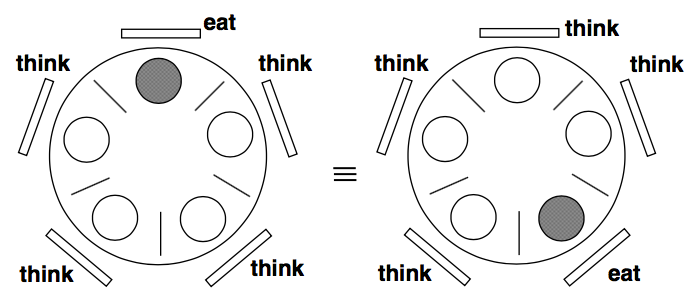
\includegraphics[width=8cm,keepaspectratio]{fig/dinning-symmetry} % Or .pdf
\caption{Symmetries and the dinning philosophers~\cite{KrenaVojnarOverview}.}
\label{fig:fav:dinning}
\end{wrapfigure}

The methods used for this include {\em symmetry reduction} in cases where it is not important which specific entity (if there is more entities of the same type is in a specific state). See \Cref{fig:fav:dinning} for an example of symmetry in the well known dinning philosophers problem.

Other solutions can be to use only one of many possible paths for the ordering of concurrent actions that are independent of each other and compress the size of states by using pointers to the previous state for values that did not change. Or the tool can evaluate the properties at the same time when a new state is generated, and stop immediately once it is clear that this prefix cannot be accepted by the automata denoting correctness specification.


%.......................
\subsubsection{CPAChecker}
%.......................

An open-source tool and a framework for an analysis of programs in C language. It is based on the idea of {\em configurable program analysis}~\cite{CPAChecker}, which uses user configuration to perform a reachability analysis.


%======================================================================
\section{Theorem Proving}\label{chap:fav:theoremProving}
%----------------------------------------------------------------------
Tools using it: VCC~\cite{KrenaVojnarOverview}, ESC/Java2~\cite{KrenaVojnarOverview}, VS3~\cite{KrenaVojnarOverview}

{\em Theorem proving} is similar to mathematical deduction, where we get a proof from an initial set of axioms. It also shares advantages and disadvantages with its purely mathematical counterpart. On the one side, it is really universal, but on the other side, it can not provide a {\em counterexample} (a path to an error), but just says yes/no, and is only semiautomatic. The tools can correctly apply inference rules, but their choice is up to the user. Thus, an insufficiently skilled user may not be able to prove that the system is correct even if there are no errors in the system.



%==================================
% (c) Jan Tulak, 2017
%%%%%%%%%%%%%%%%%%%%%%%%%%%%%%%%%%%%%%%%%%%%%%%%%%%%%%%%%%%%%%%%%%%%%%%%%%%%%

\chapter{Used Techniques and procedures}\label{chap:techniques}
%----------------------------------------------------------------------

In this chapter, we discuss which techniques and models of formal analysis and verification are useful for the code of {\tt mkfs.xfs}. Let us at first define important constraints that are limiting or directing our choice.

First of all, we are analysing a single-threaded application. This greatly reduces the state space and means that we also can use methods that do not allow for concurrency. On the other side, given that the program accepts user input, some variables has an infinite number of potential values and any method based on state space checks has to cope with this fact.

With respect to possible difficulties with implementing various advanced
methods and their required proficiency, it was decided to begin with well-known
and used tools and gradually move from these production-ready, easy to use
solutions to tools requiring more of user input.

Some tools will be used multiple times, because while, for example, {\em
	Coverity} can be used on the whole source of {\em xfsprogs}, other
	tools like {\em CPAChecker} require modelling of the environment and so
	for practical reasons, they are run only on an extracted part of {\tt
		mkfs\_xfs.c}, where things like access to disk devices are
		removed to create a maximally self-contained code. This means
		that we are not be able to detect errors in some parts of the
		code, but it is nearly impossible to model and test a whole
		operating system and we have to make the cut somewhere.

Thus, to be able to compare the various tools directly, some of the tools are run both on the full code as well as on the dissected part.

A potentially interesting comparison could be if there exist some tools using neural networks and deep learning as an integral part of their algorithms. For example as a heuristic to drive the selection of inference rules in theorem proving, or for spotting error patterns~\footnote{Some attempts in modelling a code are hinted in {\em On the Naturalness of Software} by Abram Hindle: \url{http://dl.acm.org/citation.cfm?id=2902362}.} However, these approaches are even more complex and experimental and would probably deserve a standalone work on their own.
% TODO http://dl.acm.org/citation.cfm?id=2902362 download and read... search for deep learning sources

List of tools that were used in this work (in no particular order): Coverity,
CPAChecker, CppCheck and the analysis in GCC and Clang compilers.


%======================================================================
\section{Testing Environment}\label{chap:techniques:env}
%----------------------------------------------------------------------

The tools were run in a Docker container\footnote{Simply stated, a
	container is an image that has been started, similar to the
		difference between a running virtual machine and its
		on-disk virtual HDD image. Unlike virtualization,
		containers are only processes isolated from the rest of the
system using kernel capabilities, like {\em cgroups} and {\em chroot}.
Docker is a specific implementation~\cite{docker} of containers.} based on Fedora Linux
25. The use of containers ensures a clean and identical environment for
every tool and every run. Images with CPAChecker and CppCheck are published
in Docker Hub and all the recipes to build and use them are provided with
this work. Image with Coverity could not be published, because it contains
confident information\footnote{Jan Ťulák had an access to Red Hat Coverity license
server as a Red Hat employee. However, the server information and some tools
	Red Hat provided with Coverity are considered confidential.}.


Every image has its own starting script for easier manipulation -- {\tt
run.sh}.  This script creates a container from the image and mounts the
directory with xfsprogs (or any other directory which is passed to it).
Then, if necessary, it can pass few options to the script started in
the container.

{\tt run-test.sh} is the script started by Docker after creating the container.
This script copies xfsprogs from the mounted directory to another one, so it
does not change the original repository in any way. In this copied directory
the script then starts whatever tool it is prepared for.

Users can, if they wish to do so, enter an interactive shell in the container
instead of starting the tool. Also, it is possible to skip the copying or to
run {\tt make clean}. For an automated run descripte in
\Cref{chap:techniques:processing} neither of this is necessary, but these
options are useful for manual experiments.


Coverity, GCC and Clang are run using {\tt csbuild}, a tool to plug static
analyzers into the build process~\cite{csbuildMan}. Because csbuild attempts to
use all supported analyzers it finds, the images for each tool we are testing
are modifed to contain only the single specific tool we need, but no other.
%_____________________________________________________
\subsection{CPAChecker}
%.....................................................
Docker image: {\tt jtulak/cpacheck}~\cite{dockerCPAChecker}

CPAChecker can not be run on a full source code, but requires
preprocessing~\cite{cpacheckerGettingStarted}, which has to be partially
remade for every tested revision (depending on what and how much changed),
       only selected commits were tested.
%_____________________________________________________
\subsection{CppCheck}
%.....................................................
Docker image: {\tt jtulak/cppcheck}~\cite{dockerCPPCheck}

CppCheck is also used in {\em Codacy}, an automated code review application
with Github integration. Results from Codacy are included for comparison.

Because CppCheck does not need preprocessed code, it was reasonable to use
it for every commit in my changes.

When running this tool, default configuration was used, and all types of
messages were enabled. No custom rules were used and the invocation of
CppCheck on whole {\tt xfsprogs/mkfs/} directory was:

{\tt cppcheck --enable=all mkfs/}

\TODO{Find some non-default rules for cppcheck and test with them? Or try to
	write a rule for issues found by other tools.}


%_____________________________________________________
\subsection{Coverity}
%.....................................................
Coverity was used both manually in a Docker container, and automatically,
using the public Coverity service for open source projects, which is part
of standard xfsprogs development process, to compare the results between
those two instances.

%_____________________________________________________
\subsection{GCC}
%.....................................................
The {\em GNU project C and C++ compiler} is used for compiling xfsprogs and it
has some static analysis capabilities, because it has to understand the code to
compile it. The only difference in its use from standard configuration is to
use the most strict reporting.

%_____________________________________________________
\subsection{Clang}
%.....................................................
Clang is another C/C++ compiler. It is not used by xfsprogs, but can compile
the code as well, so we can compare it with GCC and other analysis tools. To use
clang instead of GCC, we decided that the easiest way is to rename clang binary
to gcc and let xfsprogs behave as if it was gcc, rather than modify autotools
configuration.

%======================================================================
\section{Results Processing}\label{chap:techniques:processing}
%----------------------------------------------------------------------
The outputs of these tools has different syntax and verbosity, but we had to
find a way, how to compare them, both between the tools and across revisions,
     despite some of the tools finding a great amount of issues. A set of
     scripts to help both with automating the tests and with analysing was
     created.

First, there is tool {\tt parse.py}, which can automatically run all the tools
across specified revisions. It takes care of changing the revisions, starting
every docker container again and finally, it organises the outputs in a logical
way: in a specified directory, it creates a subdirectory for every revision
(using the revision's short hash as the directory name) and each such directory
then contains log files with outputs from each tool.

The output files are not modified in the first step, but to simplify their
parsing, it is useful to preprocess some of those files (namely from GCC and
							 Clang) with script
{\tt format-outputs.sh}, to remove color formatting escape sequences and
unnecessary compiler outputs.  Such data may be useful for some further
analysis, but for the next step, it would only make the parsing more complex.

In the last step, script {\tt parse.py}, when supplied with the output
directory, translates the different syntaxes into a single inner
representation, which can be then used to simply compute deltas between
different revisions.

The algorithms to complete these deltas has one known issue: if there are
multiple issues with the same message (e.g. because variable with name {\tt
				       foo} was declared, but not used, in
				       multiple functions) and later some of
these issues are fixed, the number of issues is correct, but the indicated
lines may be incorrect. This is because the script has to cope with changing
code; an issue on line X in one revision can be on line Y in another one, and
that would require employing much more complex algorithms that would use
information from git and understand which lines moved where. Thus, in such
case, the behaviour selecting specific instancies of the same kind of issue is
undefined.


The classification of issues into one of the style, error or security category
is only indicative. For GCC and Clang it is based on what specific flag for the
compiler enables reporting of any specific issue. We attempted to estimate what
consequences can these issues have in general, whether they can cause a bigger
problem, or if their greatest danger is in being misleading or not a good
practice.

From the issues found in whole xfsprogs, we configured only one compiler flag
to be detected as something else than style issue: {\tt -Wfloat-equal}.
Directly comparing two floats is not reliable due to their representation
in memory~\cite{floatsComparing}. Thus, this kind of issue is certainly
something that can work differently than expected and deserves more
attention, than, say, shadowing a global variable with local one.

This kind of issue was not found in mkfs itself and in xfsprogs, it appears
only on two places, both to set the precision of a printf. In other words,
the only occurrences of direct comparison of floats are intentional testing
for imprecise numbers and can be considered false positives in the context
of the program. Clang finds this issue as well. In comparison, Coverity
does not raise it and it seems that it can somehow infer the intention of
the use.

For CppCheck, the classification uses the category reported by CppCheck itself:
If CppCheck reports an issue as anything else than style issue, it is
considered a potential error, but it did not report anything else than style
issue. Coverity reports also a categorization. In xfsprogs, the only two
categories that were reported are quality and security.

Finally, while it is possible to find differences between revisions within the
results of a single tool, albeit with the small instability in case of multiple
similar entries mentioned above, doing this between tools on a single revision
proved a much more complex task. Every tool describes the same issue with
different words, so to be able to automatically compute any differences, such
an algorithm would have to understand the issue in all details. Thus,
   cross-tool differences are not computed automatically, but manually for the
   cases where it is reasonable given to the amount of issues that has to be
   analysed.

%==================================
% (c) Jan Tulak, 2017
%%%%%%%%%%%%%%%%%%%%%%%%%%%%%%%%%%%%%%%%%%%%%%%%%%%%%%%%%%%%%%%%%%%%%%%%%%%%%

\chapter{Results}\label{chap:results}
%----------------------------------------------------------------------

If not stated otherwise, the number of issues is for mkfs-specific files.
That is, for files in {\tt mkfs/} directory.

\begin{table}[h]
\begin{tabular}{|r||r|r|r|r|r|r|}
\hline
Commit & CppCheck & Codacy & CPAChecker & Coverity & GCC & Clang \\
\hline
\hline
\multicolumn{7}{|c|}{Total issues}\\
\hline
(tag: v4.11.0-rc1) {\tt 07a3e793} & $1$ & $3$ & & & $30$ & $34$ \\
\hline
(tag: v4.7.0) {\tt d7e1f5f1} & $1$ & $4$ & & & $30$ & $28$ \\
\hline
\hline
\multicolumn{6}{|c|}{Changes}\\
\hline
{\em [Last of my set]} {\tt 2aca16d6} & 0 & 0 & & & 0 & 0 \\
\hline
{\tt aa3034d4} & 0 & 0 & & & 0 & 0 \\
\hline
{\tt 6de2e6c0} & 0 & 0 & & & 0 & 0 \\
\hline
{\tt ddc3b2da} & 0 & 0 & & & 0 & 0\\
\hline
{\tt 06ac92fd} & 0 & 0 & & & $+1$ & $+1$\\
\hline
{\tt 27ae3a59} & 0 & 0 & & & 0 & 0 \\
\hline
{\tt 3ec1956a} & 0 & 0 & & & 0 & 0 \\
\hline
{\tt 6c855628} & 0 & 0 & & & $-2$ & $-2$ \\
\hline
{\tt 627e74fd} & $-3$ & $-2$ & & & $+2$ & $+2$ \\
\hline
{\tt 9090e187} & 0 & 0 & & & 0 & 0 \\
\hline
{\tt 1974d3f1} & 0 & 0 & & & $-1$ & 0 \\
\hline
{\tt 56e4d368} & 0 & 0 & & & 0 & 0 \\
\hline
{\tt a9dad670} & 0 & 0 & & & $-54$ & $-54$ \\
\hline
{\tt 147e0f31} & 0 & 0 & & & 0 & 0 \\
\hline
{\tt c81c8460} & 0 & 0 & & & $-50$ & $-50$ \\
\hline
{\tt a887c950} & 0 & 0 & & & $+13$ & $+12$ \\
\hline
{\tt 5f1a2100} & 0 & 0 & & & 0 & 0 \\
\hline
{\tt ff21c709} & 0 & 0 & & & $+1$ & $+1$ \\
\hline
{\em [First of my set]} {\tt 4a32b9e9} & $-1$ & 0 & & & 0 & 0 \\
\hline
\hline
\multicolumn{7}{|c|}{Total issues} \\
\hline
{\em [Before my set]} {\tt 6aa32b47} & $5$ & $6$ & & & $121$ & $117$ \\
\hline
(4.6.0) {\tt 09033e35} & $5$ & $6$ & & & $121$ & $117$ \\
\hline
\end{tabular}
\caption{An overview of issues found by the tested tools on specific
	revisions in mkfs-only files.\newline
	\newline
	Legend: Revisions annotated with {\em total issues} shows the
	number of outstanding issues. All other revisions shows new/fixed
	issues.  $+x$ denotes amount of new issues found, $-x$ denotes number
	of issues fixed between this and the previously tested revision. The
	numbers are absolute, that is, 0 means no change, $+1$ means one new
	issue and $+1$/$-2$ means one new and two removed. A --- dash means that
	the tool was not used on this specific revision.}


\label{tab:results:overview}
\end{table}

%======================================================================
\section{CppCheck}\label{chap:results:cppcheck}
%----------------------------------------------------------------------



%======================================================================
\section{Codacy}\label{chap:results:codacy}
%----------------------------------------------------------------------
Codacy shows only per-commit and total issues for a branch. That is, a
developer can view whether a specific commit fixed or caused an issue, and
can see what are the issues for the top of the repository, but checking the
complete state on a particular point in the history requires creating a new
branch, which is uncomfortable, but manageable for a private\footnote{In
the sense of being the only user, not in terms of visibility.} repository.
In a repository with many contributors it can be confusing.

% ------------------------------------------------
\subsection{Version {\tt 4.11-rc1}}
An overview of issues at this revision.
\begin{table}[h]
\begin{tabular}{|l||r|r||r|}
\hline
& {\tt mkfs/xfs\_mkfs.c} & {\tt mkfs/proto.c} & Whole xfsprogs \\
\hline
Issues & 1 & 2 & 937 \\
\hline
\end{tabular}
\caption{In mkfs-specific files, 3 issues were found. Whole
xfsprogs had 937 issues, from which 900 were code style issue, 36 were
potential errors and 1 was a security issue.}
%\label{tab:results:overview}
\end{table}

The issues found in mkfs are:
\begin{enumerate}
	\item {\tt mkfs/xfs\_mkfs.c}: The scope of the variable 'bucket' can be reduced.
	\item {\tt mkfs/proto.c}: The function 'setup\_proto' is never used.
	\item {\tt mkfs/proto.c}: The function 'parse\_proto' is never used.
\end{enumerate}

% ------------------------------------------------
\subsection{Version 4.7}
An overview of issues at this revision.
\begin{table}[h]
\begin{tabular}{|l||r|r|r||r|}
\hline
& {\tt mkfs/xfs\_mkfs.c} & {\tt mkfs/maxtrres.c} & {\tt mkfs/proto.c} & Whole xfsprogs \\
\hline
Issues & 1 & 1 & 2 & 749 \\
\hline
\end{tabular}
\caption{In mkfs-specific files, 4 issues were found. Whole
xfsprogs had 749 issues, from which 719 were code style issue and 30 were
potential errors.}
%\label{tab:results:overview}
\end{table}

The issues found in mkfs are:
\begin{enumerate}
	\item {\tt mkfs/xfs\_mkfs.c}: The scope of the variable 'bucket' can be reduced.
	\item {\tt mkfs/maxtrres.c}: The function 'max\_trans\_res' is never used.
	\item {\tt mkfs/proto.c}: The function 'setup\_proto' is never used.
	\item {\tt mkfs/proto.c}: The function 'parse\_proto' is never used.
\end{enumerate}

% ------------------------------------------------
\subsection{Version 4.6}

An overview of issues at this revision.
\begin{table}[h]
\begin{tabular}{|l||r|r||r|}
\hline
& {\tt mkfs/xfs\_mkfs.c} & {\tt mkfs/proto.c} & Whole xfsprogs \\
\hline
Issues & 4 & 2 & 839 \\
\hline
\end{tabular}
\caption{In mkfs-specific files, 6 issues were found. Whole
xfsprogs had 839 issues, from which 809 were code style issue and 30 were
potential errors.}
%\label{tab:results:overview}
\end{table}

The issues found in mkfs are:
\begin{enumerate}
	\item {\tt mkfs/xfs\_mkfs.c}: Checking if unsigned variable 'blocksize' is less than zero.
	\item {\tt mkfs/xfs\_mkfs.c}: Checking if unsigned variable 'sectorsize' is less than zero.
	\item {\tt mkfs/xfs\_mkfs.c}: Condition '0' is always false
	\item {\tt mkfs/xfs\_mkfs.c}: The scope of the variable 'bucket' can be reduced.
	\item {\tt mkfs/proto.c}: The function 'setup\_proto' is never used.
	\item {\tt mkfs/proto.c}: The function 'parse\_proto' is never used.
\end{enumerate}

All these issues were present for multiple years. Precise dating is
difficult, however, because e.g. issue 1. is blamed for a commit 16 years
old. But at that time, the variable was signed. Thus, the issue appeared
some time later, when the specific variable was turned to unsigned, but not
every use was fully converted.



% ------------------------------------------------
\subsection{Revision 627e74fd}
Fixed 2 issues in {\tt mkfs/xfs\_mkfs.c}:

\begin{enumerate}
\item Checking if unsigned variable 'blocksize' is less than zero. (line 1579)
\item Checking if unsigned variable 'sectorsize' is less than zero. (line
								     1705)
\end{enumerate}

\subsection{Summary}
Codacy provides some rating on the project's page~\cite{codacyXfsprogs},
which considers xfsprogs as a quality project (A-grade).

\TODO{compare with other tools}

%======================================================================
\section{CPAChecker}\label{chap:results:cpachecker}
%----------------------------------------------------------------------

%======================================================================
\section{Coverity}\label{chap:results:coverity}
%----------------------------------------------------------------------

%======================================================================
\section{GCC}\label{chap:results:gcc}
%----------------------------------------------------------------------

%======================================================================
\section{Clang}\label{chap:results:clang}
%----------------------------------------------------------------------



\chapter{Conclusion} \label{chap:conclusion}

At this moment, in January 2017, the refactoring is probably mostly finished. About half of the changes is already in the upstream repository, while the other half awaits review. The review process can take some time as it is likely that there will be multiple iterations, but I don't expect any big changes.

Once all the changes are merged, I can begin the testing, with one notable exception: Coverity scan is used during the development because xfsprogs is using the Coverity Scan program for open-source projects.


 % viz. obsah.tex

  % Pouzita literatura
  % ----------------------------------------------
\ifczech
  \bibliographystyle{czechiso}
\else 
  \bibliographystyle{plain}
%  \bibliographystyle{alpha}
\fi
  \begin{flushleft}
  \bibliography{bibliography} 
  \end{flushleft}


%\chapter*{Appendices}
foo


\end{document}
